\section{Acceleration}\label{sectionAcceleration_new}
After many tests, and implementation it was possible to add another discrete action - the acceleration. Instead of the car driving at a constant speed as seen in \Cref{sectionAcceleration}, the agent can learn how to accelerate the car. This gives a more realistic view of the car simulation because humans don't just drive at a constant speed all the time, sometimes it is better to drive fast, and sometimes it is better to drive slow.  

The acceleration is a discrete action, but it is a discrete action the car should learn, to be able to drive a lap. The most optimal parameter for the acceleration needs to be found. The acceleration is a number between 0 and 1, where 0 means no throttle and 1 is full throttle. It is thereby the throttle in the car which decides the acceleration, and it is the throttle which is the discrete action.

The different acceleration/throttle values tested as a discrete action is:

\begin{itemize}
	\item 0.1
	\item 0.2
	\item 0.4
\end{itemize} 
   
If the acceleration is bigger the car will accelerate faster - the speed will increase faster. Because no break action is implemented, this means if the car has a bigger acceleration, the speed, in general, will be bigger. 

To see if the agent is able to learn how to drive, a graph of the total reward is seen on \Cref{fig:change_of_acceleration_new_reward_graph}.

\begin{figure}[H]
	\centering
	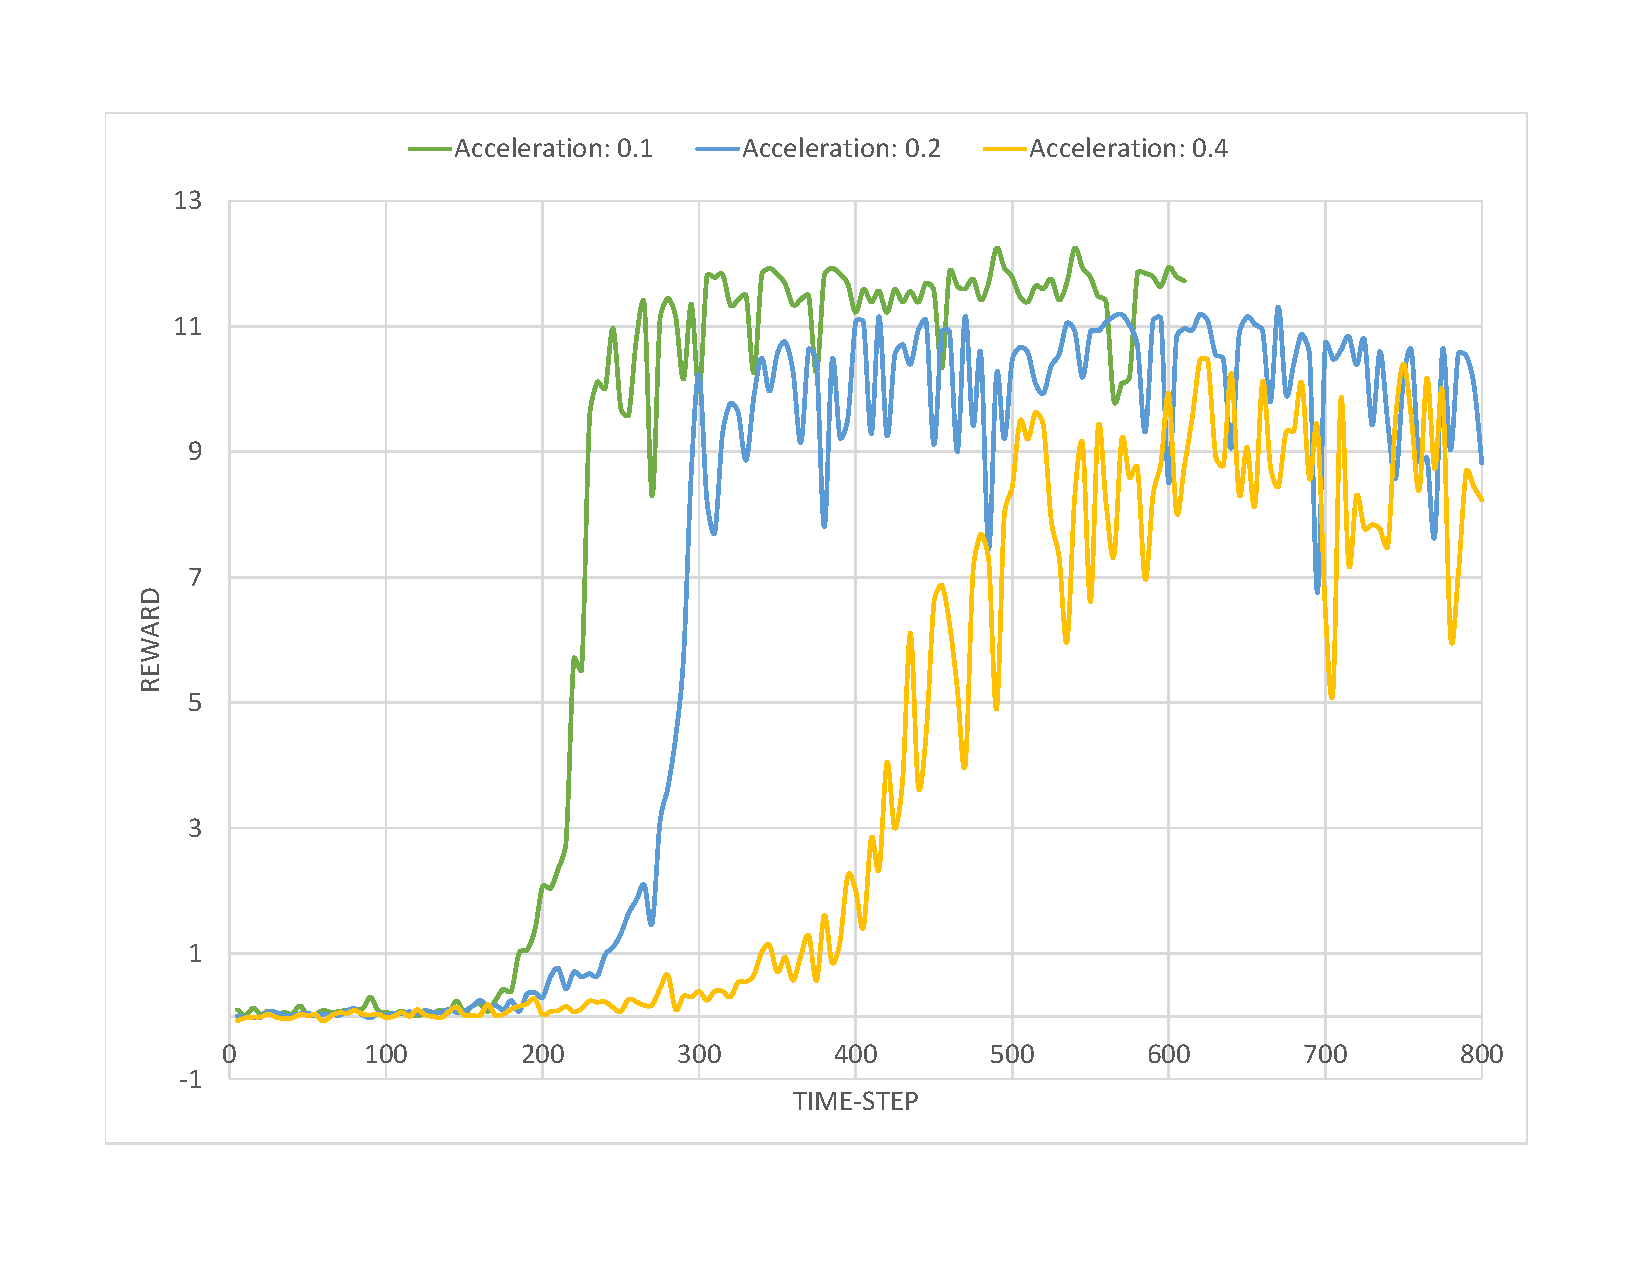
\includegraphics[width=1\textwidth]{Figures/Result/change_of_acceleration_new_reward_graph.pdf}
	\caption{Comparison of the three different accelerations with the reward getting from the environment}
	\label{fig:change_of_acceleration_new_reward_graph}
\end{figure} 

On \Cref{fig:change_of_acceleration_new_reward_graph} it is seen that all the different acceleration values converge to a reward value. In the graph, it looks like the agent has learned how to drive the car a lap. This is also the conclusion by looking at the car in the TORCS environment. 

The reward is higher with an acceleration of 0.1 than with accelerations of 0.2 or 0.4. This is since it drives slower, it uses more steps to finish the lap, and the total reward is equal to the reward in all the steps added together. This is not seen as a problem in this project, because it is only needed to learn how to drive a lap, and not to drive it fast, and all the accelerations learn how to drive a lap.

The stability is different for the different accelerations. Here it is more stable with an acceleration of 0.1 instead of 0.2 or 0.4. This can be because of the discrete value for steering as mention in \Cref{sectionAcceleration}. The discrete steering values are optimized to a speed of 10 km/h. Sometimes the speed reaches 60 km/h with an acceleration of 0.4, the steering values should then be changed.  

Looking at the training time, it looks like it is learning slower with an acceleration of 0.4 than with 0.2 and 0.1. This is the same problem with the speed in \Cref{sectionAcceleration}. With an acceleration of 0.4, the time-steps finish faster, so it takes more time-steps to learn. To get a better view of the training time, a graph with training time in hours instead of time-steps is created. This graph can be seen on \Cref{fig:change_of_acceleration_new_reward_hours_graph}.       

\begin{figure}[H]
	\centering
	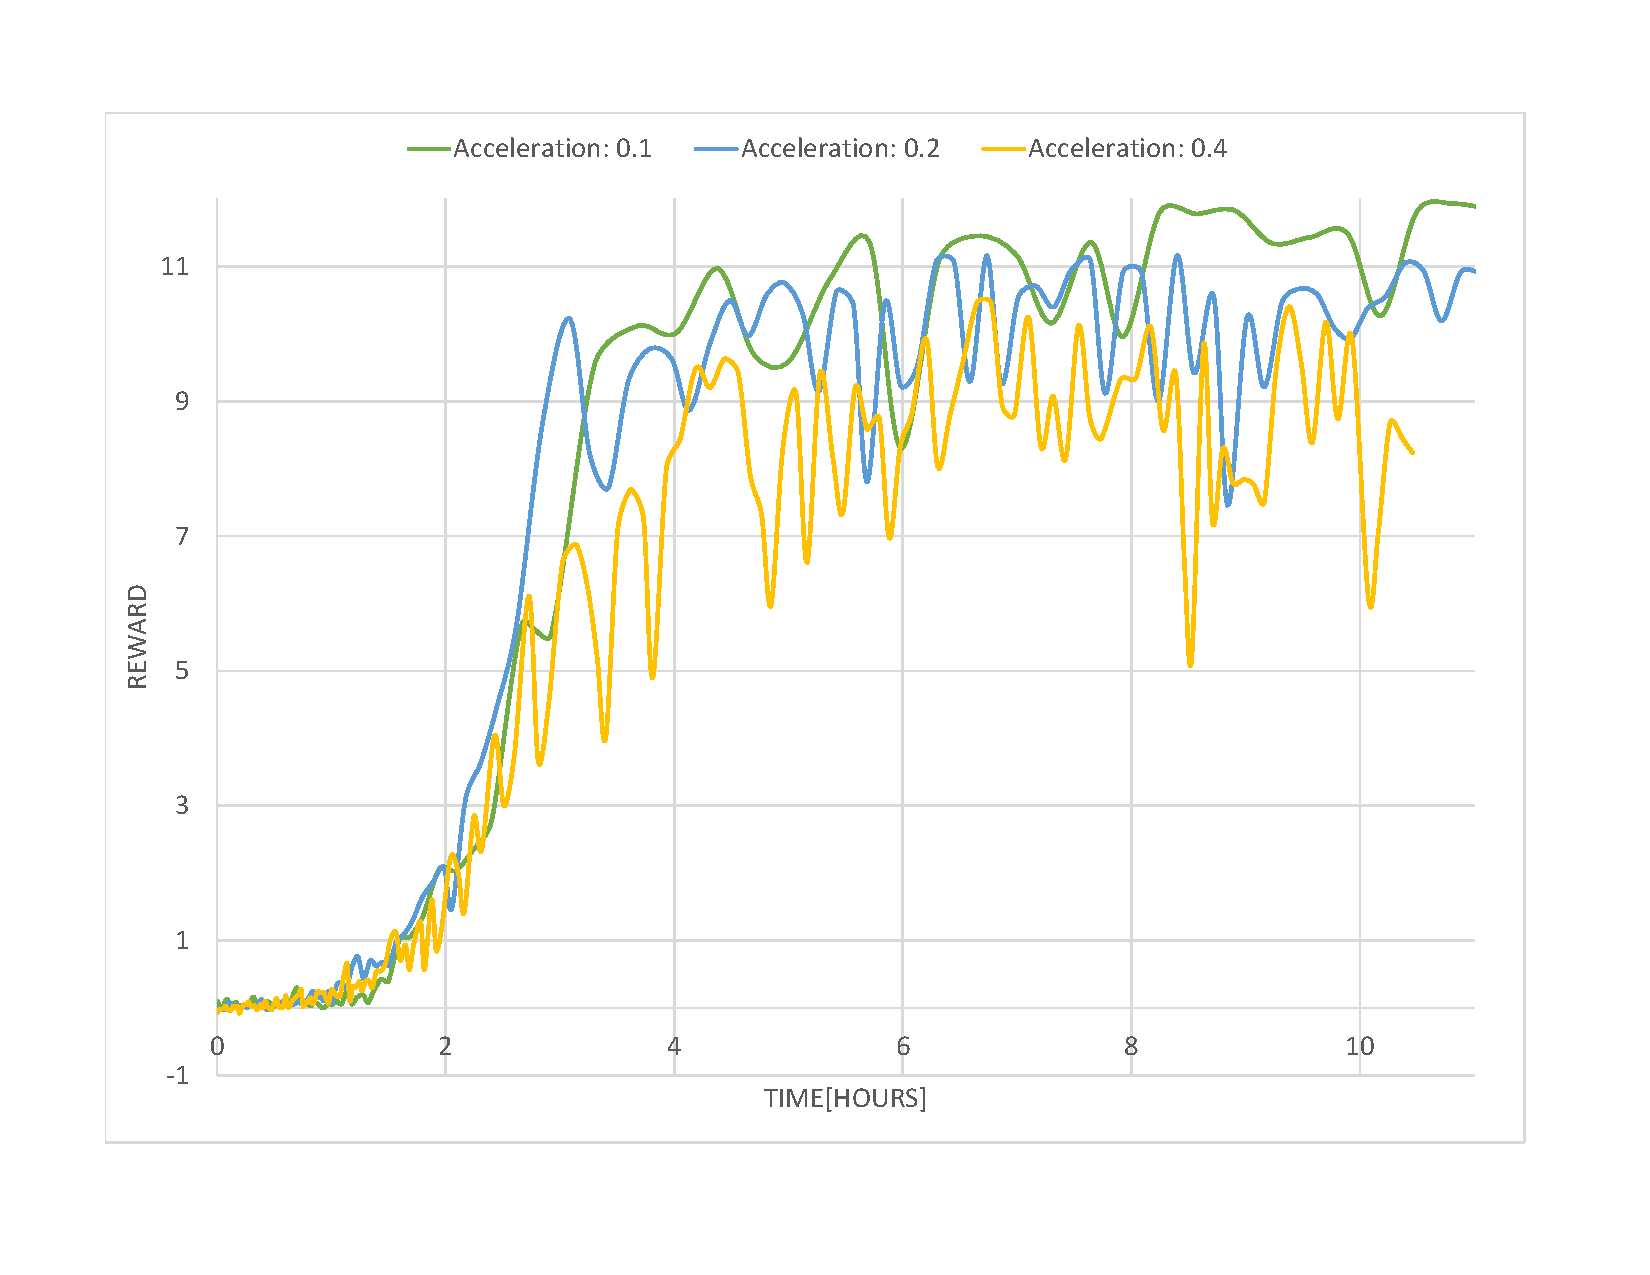
\includegraphics[width=1\textwidth]{Figures/Result/change_of_acceleration_new_reward_hours_graph.pdf}
	\caption{Comparison of the three different accelerations with the reward getting from the environment. Here it is the time in hours, instead of time-steps on the x-axis}
	\label{fig:change_of_acceleration_new_reward_hours_graph}
\end{figure}

On \Cref{fig:change_of_acceleration_new_reward_hours_graph} It is seen the training time is the same for all accelerations - around 3 hours. 

Most of the result in this \Cref{cha:Result} is done without the acceleration as an action, due to the timescale of the project, this action was implemented late in the project. If more testing should be done in the future, it is concluded that acceleration as an action would work without problems.   